\documentclass[aspectratio=169]{beamer}

% ==== Theme & basic look ====
\usetheme{Madrid}
\usecolortheme{seahorse}
\setbeamertemplate{navigation symbols}{}
\setbeamertemplate{footline}[frame number]


% Packages for mathematics  
\usepackage{amsmath}  
\usepackage{amsfonts}  
\usepackage{amssymb}  
\usepackage{CJKutf8}
% Support for \Tilde macro used throughout
\providecommand{\Tilde}[1]{\tilde{#1}}
\providecommand{\proofname}{Proof}
\newenvironment<>{proofs}[1][\proofname]{%
    \par
    \def\insertproofname{#1.}%
    \usebeamertemplate{proof begin}#2}
  {\usebeamertemplate{proof end}}
\makeatother

% Math shorthand and vector symbols
\newcommand{\grad}{\nabla}
\newcommand{\EE}{\mathbb{E}}
\newcommand{\dd}{\mathrm{d}}
\newcommand{\kbT}{k_B T}
\newcommand{\vx}{\mathbf{x}}
\newcommand{\bm}{\mathbf}

% Bold vector/time-indexed variables
\newcommand{\vxz}{\mathbf{x}_0}
\newcommand{\vxt}{\mathbf{x}_t}
\newcommand{\alpt}{\alpha_t}
\newcommand{\sigt}{\sigma_t}
\newcommand{\veps}{\boldsymbol{\epsilon}}
\newcommand{\vF}{\mathbf{F}}

% Title page details:   
\title[Understanding diffusion model]{Understanding diffusion model from a mathematical view}  
\author{Pipi Hu}  
\institute[BIMSA]{Beijing Institute of Mathematical Sciences and Applications}  
\date{\today}  

\pgfdeclareimage[width=2cm]{logo}{figs/logo.png}
\logo{\pgfuseimage{logo}}

% Outline slide (moved to later; avoid frame before \begin{document})

\setbeamertemplate{navigation symbols}{}
\AtBeginSection[]  
{  
    \begin{frame}<beamer>{Outline}         
        \tableofcontents[currentsection]  
    \end{frame}  
}  
  
\AtBeginSubsection[]  
{  
    \begin{frame}<beamer>{Outline}         
        \tableofcontents[currentsection,currentsubsection]  
    \end{frame}  
}  

% \setbeamertemplate{navigation symbols}{}
% \AtBeginSection[]
% {
%     \begin{frame}<beamer>{Outline}       \tableofcontents[currentsection]
%     \end{frame}
% }

\begin{document}  
  
% Title slide  
\begin{frame}  
  \titlepage  
\end{frame}  

\begin{frame}{Feynman's words}
\centering
    What I cannot create, I do not understand.
\end{frame}
  
% Presentation slides  



\section{Preliminary: Generating Samples from Probability Distributions}

\begin{frame}{Generate samples from given distribution}
Given a distribution $p(x)$, how to sample from the distribution?
\begin{itemize}
    \item Uniform distribution \& Gaussian distribution: easy sampling 
    \item Mixture Gaussian: determine which Gaussian to sample \& sample from that Gaussian
    \item A general sample function?
    \begin{itemize}
        \item \textcolor{red}{Langevin Markov Chain Monte Carlo sampling (Langevin MCMC)}
        \item Stein Variational Gradient Descent (SVGD)
        \item ...
    \end{itemize}
\end{itemize}
\end{frame}

\begin{frame}{Score function is all you need?}
A typical process of generating new samples from modeling the data distribution
    \begin{enumerate}
        \item To find the probability function $p(x)$, model $p(x;\theta)$.
        \item Normalization distribution $p(x;\theta)=\frac{1}{C(\theta)}e^{-E(x;\theta)}$ with $C(\theta)\equiv\int_x e^{-E(x;\theta)}dx$.
        \item Generating samples from above sampling methods.
    \end{enumerate}
Recall the Langevin Markov Chain Monte Carlo sampling
\begin{equation}
    x_t = x_{t-1}+\frac{\Delta t}{2}\textcolor{red}{\nabla_x\log p(x_{t-1};\theta)}+\sqrt{\Delta t}\epsilon, \quad \epsilon\sim N(0, 1).
\end{equation}
Here $\textcolor{red}{\nabla_x\log p(x_{t-1};\theta)}=-\nabla_xE(x;\theta)$ is free of the normalization $C(\theta)$.

Define the score function
\begin{equation}
    S(x;\theta) \equiv \textcolor{red}{\nabla \log p(x;\theta)}.
\end{equation}
\end{frame}

\begin{frame}{More about Langevin MCMC and the score function}
Continuous form of the Langevin MCMC
\begin{itemize}
    \item $\Delta t\to 0$
    \begin{equation}
        dx = \frac{1}{2}\nabla_x\log p(x) dt+ dB_t,
    \end{equation}
    where $dB_t$ is a Brownian motion.
    \item Given $p(x)=\frac{1}{C}e^{-E}$, we have 
    \begin{equation}
        dx = -\frac{1}{2}\textcolor{red}{\nabla_x E}dt + dB_t
    \end{equation}
\end{itemize}
Langevin MCMC is  overdamped Langevin dynamics
\begin{itemize}
    \item Langevin dynamics (MD)
    \begin{equation}
        \ddot{x} = -\nabla_x E - \gamma \dot{x} + dB_t,
    \end{equation}
    \item Given $\gamma \dot{x}
    \gg \ddot{x}$, we have the overdamped Langevin equation 
    \begin{equation}
        dx = -\frac{1}{\gamma}\nabla_x E + \frac{1}{\gamma}dB_t.
    \end{equation}
\end{itemize}
\end{frame}

\section{Matching score for training}
\begin{frame}{Matching the score by neural networks}
Recall the definition 
\begin{equation}
    S \equiv \nabla_x\log p(x),
\end{equation}
The key is to matching the score by a neural network
\begin{equation}
    J_{ESM} =\frac{1}{2} \mathbb{E}_p\left[\|s(x;\theta)-\frac{\partial \log p(x)}{\partial x}\|^2\right],
\end{equation}
where $J_{ESM}$ is called Explicit Score Matching loss. However, it is not tractable to compute $\frac{\partial \log p(x)}{\partial x}$ from data.\\[1em]

Where should we go?
\end{frame}

\begin{frame}{Implicit Score Matching (ISM) loss}
Implicit Score Matching loss (Aapo, 2005) was developed to make a tractable score matching 
\begin{equation}
    J_{ISM} \equiv \mathbb{E}_p\left[\frac{1}{2}\|s(x;\theta)\|^2+\nabla\cdot s(x;\theta)\right]=J_{ESM}-C.
\end{equation}
\end{frame}

\begin{frame}{ISM Proof: Expansion of ESM}
\begin{proof}
First, we expand the ESM loss:
\begin{equation}
    J_{ESM}=\frac{1}{2} \mathbb{E}_p\left[\|s(x;\theta)-\frac{\partial \log p(x)}{\partial x}\|^2\right]
\end{equation}
\begin{equation}
    = \frac{1}{2} \mathbb{E}_p\left[\|s\|^2\right]- \mathbb{E}_p[s\cdot\frac{\partial \log p}{\partial x}] + \frac{1}{2}\mathbb{E}_p\left[\|\frac{\partial \log p}{\partial x}\|^2\right]
\end{equation}
The key insight is to simplify the cross term using integration by parts.
\end{proof}
\end{frame}

\begin{frame}{ISM Proof: Integration by Parts}
\begin{proofs}[\proofname\ (Cont)]
The cross term can be simplified:
\begin{equation}
    -  \mathbb{E}_p[s\cdot\frac{\partial \log p}{\partial x}] =-\int_x ps\cdot \nabla \log p dx
\end{equation}
\begin{equation}
    = -\int_x ps\cdot \frac{\nabla p}{p}dx = -\int_x s\cdot \nabla pdx
\end{equation}
\begin{equation}
    = -\int \nabla\cdot(ps)dx + \int p\nabla\cdot sdx=\mathbb{E}_p[\nabla\cdot s]
\end{equation}
\end{proofs}
\end{frame}

\begin{frame}{ISM Proof: Final Result}
\begin{proofs}[\proofname\ (Cont)]
Therefore, we have:
\begin{equation}
    J_{ISM}= J_{ESM}-C
\end{equation}
where $C \equiv \frac{1}{2}\mathbb{E}_p\left[\|\frac{\partial \log p}{\partial x}\|^2\right]$ is a constant independent of $\theta$.

This makes ISM tractable since we don't need to compute the true score function.
\end{proofs}
\end{frame}

\begin{frame}{Denoising Score Matching (DSM) loss}
However, the ISM score is not very stable to optimize, with two reasons
\begin{enumerate}
    \item Expectation is performed on the whole distribution;
    \item The loss is negative decreasing to $-C$ with a great quantity, e.g. $-1e5$.
\end{enumerate}

Denoising Score Matching (DSM) loss (Vincent, 2011) is developed to solve this problem
\begin{equation}
    J_{DSM} = \frac{1}{2}\mathbb{E}_{p(x,\Tilde{x})}\left[\|s(\Tilde{x};\theta)-\nabla_{\Tilde{x}}\log p(\Tilde{x}|x)\|^2\right].
\end{equation}
And we can prove that $J_{DSM} = J_{ESM}+C$.
\end{frame}

\begin{frame}{DSM Proof: Expansion}
\begin{proof}
We expand the DSM loss:
\begin{equation}
    J_{DSM} \equiv \frac{1}{2}\mathbb{E}_{p(x,\Tilde{x})}\left[\|s(\Tilde{x};\theta)-\nabla_{\Tilde{x}}\log p(\Tilde{x}|x)\|^2\right]
\end{equation}
\begin{equation}
    =\frac{1}{2}\mathbb{E}_{p(\Tilde{x})}\left[\|s(\Tilde{x})\|^2\right]-\mathbb{E}_{p(x,\Tilde{x})}[s(\Tilde{x})\cdot\nabla_{\Tilde{x}}\log p(\Tilde{x}|x)]
\end{equation}
\begin{equation}
    +\frac{1}{2}\mathbb{E}_{p(x,\Tilde{x})}[\|\nabla_{\Tilde{x}}\log p(\Tilde{x}|x)\|^2]
\end{equation}
The key step is to show that the cross terms of $J_{ESM}$ and $J_{DSM}$ are equal.
\end{proof}
\end{frame}

\begin{frame}{DSM Proof: Cross Term Equivalence}
\begin{proofs}[\proofname\ (Cont)]
We need to show:
\begin{equation}
    \mathbb{E}_p(\Tilde{x})[s(\Tilde{x})\cdot\nabla_{\Tilde{x}}\log p(\Tilde{x})] = \mathbb{E}_{p(\Tilde{x},x)}\left[s(\Tilde{x})\cdot\nabla_{\Tilde{x}} \log p(\Tilde{x}|x)\right]
\end{equation}
Starting from the left side:
\begin{equation}
    = \int_{\Tilde{x}} p(\Tilde{x})s(\Tilde{x})\cdot\nabla_{\Tilde{x}}\log p(\Tilde{x})d\Tilde{x}
\end{equation}
\begin{equation}
    = \int_{\Tilde{x}} s(\Tilde{x})\cdot\nabla_{\Tilde{x}} p(\Tilde{x})d\Tilde{x}
\end{equation}
\end{proofs}
\end{frame}

\begin{frame}{DSM Proof: Cross Term Equivalence (Cont)}
\begin{proofs}[\proofname\ (Cont)]
Continuing the derivation:
\begin{equation}
    = \int_{\Tilde{x}}\int_x p(x)s(\Tilde{x})\cdot\nabla_{\Tilde{x}} p(\Tilde{x}|x)d\Tilde{x}dx
\end{equation}
\begin{equation}
    = \int_{\Tilde{x}}\int_x p(\Tilde{x}|x)p(x)s(\Tilde{x})\cdot\nabla_{\Tilde{x}} \log p(\Tilde{x}|x)d\Tilde{x}dx
\end{equation}
\begin{equation}
    = \mathbb{E}_{p(\Tilde{x},x)}\left[s(\Tilde{x})\cdot\nabla_{\Tilde{x}} \log p(\Tilde{x}|x)\right]
\end{equation}
This completes the proof of cross term equivalence.
\end{proofs}
\end{frame}

\begin{frame}{DSM Proof: Final Result}
\begin{proofs}[\proofname\ (Cont)]
Therefore, we have:
\begin{equation}
    J_{DSM} = J_{ESM} -\frac{1}{2}\mathbb{E}_p\left[\|\nabla_{\Tilde{x}} \log p(\Tilde{x})\|^2\right] + \frac{1}{2}\mathbb{E}_{p(x,\Tilde{x})}[\|\nabla_{\Tilde{x}}\log p(\Tilde{x}|x)\|^2]
\end{equation}
Since the last two terms are constants independent of $\theta$, we have $J_{DSM} = J_{ESM} + C$ where $C$ is a constant.
\end{proofs}
\end{frame}

\begin{frame}{DSM is all you need?}
Problem arises when $\Tilde{x}\to x$. 
We can prove that when Gaussian noised added by  $p(\Tilde{x}|x) = N(\alpha x, \sigma^2)$, 
\begin{equation}
    J_{DSM}\to \infty, \text{ if } \Tilde{x}\to x.
\end{equation}
\begin{proof}
  Given the Gaussian noise added, we have \\[-1em] 
  \begin{equation}
\nabla_{\Tilde{x}}\log p(\Tilde{x}|x) = \nabla_{\Tilde{x}}\log e^{-\frac{(\Tilde{x}-\alpha x)^2}{2\sigma^2}} = -\frac{\Tilde{x}-\alpha x}{\sigma^2}.
  \end{equation}  
And we can show that the following formula goes to infinity\\[-1em]
\begin{equation}
\begin{aligned}
&\mathbb{E}_{p(x,\Tilde{x})}[\|\nabla_{\Tilde{x}}\log p(\Tilde{x}|x)\|^2] 
=\mathbb{E}_{p(x,\Tilde{x})}[\|\frac{\Tilde{x}-\alpha x}{\sigma^2}\|^2]\\
&=\mathbb{E}_{p(x)}\mathbb{E}_{p(\Tilde{x}|x)}[\|\frac{\Tilde{x}-\alpha x}{\sigma^2}\|^2]
=\mathbb{E}_{\epsilon\sim N(0,1)}[\|\frac{\epsilon}{\sigma}\|^2] \to \infty \text{ if } \sigma\to 0.
\end{aligned}
\end{equation}
Finally, we know that\\[-1em]
\begin{equation}
    J_{DSM} = J_{ESM}+C \to \infty \text{ as } C\to \infty \text{ when } \Tilde{x}\to x.
\end{equation}
\end{proof}  
\end{frame}

\section{Relations of different models: x0, epsilon and score model}

\begin{frame}{Revisit the adding noise from $x$ to $\Tilde{x}$}
Gaussian transition kernel for adding noise from $x$ to $\Tilde{x}$
\begin{equation}
    \Tilde{x} = \alpha x + \sigma \epsilon,
\end{equation}
which equivalent to the Gaussian transition kernel
\begin{equation}
    p(\Tilde{x}|x) = N(\Tilde{x}; \alpha x, \sigma^2),
\end{equation}
where $\epsilon\sim N(0,1)$ and 
\begin{equation}
    N(\Tilde{x};\alpha x, \sigma^2) = C e^{-\frac{\|\Tilde{x}-\alpha x\|^2}{2\sigma^2}}.
\end{equation}
And 
\begin{equation}
    \epsilon = \frac{\Tilde{x}-\alpha x}{\sigma}.
\end{equation}\\[1em]

Questions arise: how can we get $x$ given $\Tilde{x}$?
\end{frame}

\begin{frame}{Tweedie's Formula}
    Tweedie's Formula (Bayes statistics) states (Robbins, 1956)
    \begin{theorem}
        Given random variables $x, y$, $y\sim N(x, \sigma^2I)$, i.e., $p(y|x) = N(x, \sigma^2)$, the expectation of $x$ could be given by 
        \begin{equation}
            \mathbb{E}[x|y] = y +\textcolor{red}{\sigma^2}\nabla \log p(y).
        \end{equation}
    \end{theorem}

Let
\begin{equation}
   x \leftarrow \alpha x, \quad y \leftarrow \Tilde{x},
\end{equation}
we have 
\begin{equation}
    s\equiv \nabla_{\Tilde{x}} \log p(\Tilde{x}) = -\frac{\Tilde{x}-\alpha \mathbb{E}[x|\Tilde{x}]}{\sigma^2}= -\frac{1}{\sigma}\mathbb{E}[\frac{\Tilde{x}-\alpha x}{\sigma}|\Tilde{x}] = -\frac{\mathbb{E}[\epsilon|\Tilde{x}]}{\sigma},
\end{equation}
where we have used the fact
$\epsilon = \frac{\Tilde{x}-\alpha x}{\sigma}.$

\end{frame}

\begin{frame}{Another insight: from the definition of the score $S$}
    Recall that adding noise by
    $\Tilde{x} = \alpha x + \sigma \epsilon$,
\begin{equation}\label{eq:cond}
    p(\Tilde{x}|x) = Ce^{-\frac{\|\Tilde{x}-\alpha x\|^2}{2\sigma^2}}.
\end{equation}
Hence
\begin{equation}
    s(\Tilde{x}) = \nabla_{\Tilde{x}}\log p(\Tilde{x}) = \frac{\nabla_{\Tilde{x}}p(\Tilde{x})}{p(\Tilde{x})}=\frac{\int_x \nabla_{\Tilde{x}}p(\Tilde{x}|x) p(x)dx}{p(\Tilde{x})},
\end{equation}
From Eq. \eqref{eq:cond}, we have
\begin{equation}
s(\Tilde{x}) = \frac{\int_x \nabla_{\Tilde{x}} \log p(\Tilde{x}|x)p(\Tilde{x}|x) p(x)dx}{p(\Tilde{x})} = \int_x \nabla_{\Tilde{x}} \log p(\Tilde{x}|x)p(x|\Tilde{x})dx, 
\end{equation}
leading to
\begin{equation}
s(\Tilde{x}) = \mathbb{E}_x[\nabla_{\Tilde{x}} \log p(\Tilde{x}|x)| \Tilde{x}]=\mathbb{E}_x[-\frac{\Tilde{x}-\alpha x}{\sigma^2}| \Tilde{x}] = -\frac{\Tilde{x}-\alpha \mathbb{E}[x|\Tilde{x}]}{\sigma^2}.
\end{equation}
\end{frame}

\begin{frame}{Theoretical Support: Conditional Expectation}
\begin{theorem}
\label{thm:conditional_expect}
    Let $X$ be an integrable random variable. Then for each $\sigma$-algebra $\mathcal{V}$ and $Z \in \mathcal{V}$, $Z^* = \mathbb{E}(X| \mathcal{V})$ solves the least square problem %\cite{evans2012introduction}
    $$\text{argmin}_{Z\in \mathcal{V}} \| Z - X\|\,,$$
    where $\| Z\| = \left( \int Z^2 dP \right)^{\frac{1}{2}}$.
\end{theorem}

\begin{figure}
    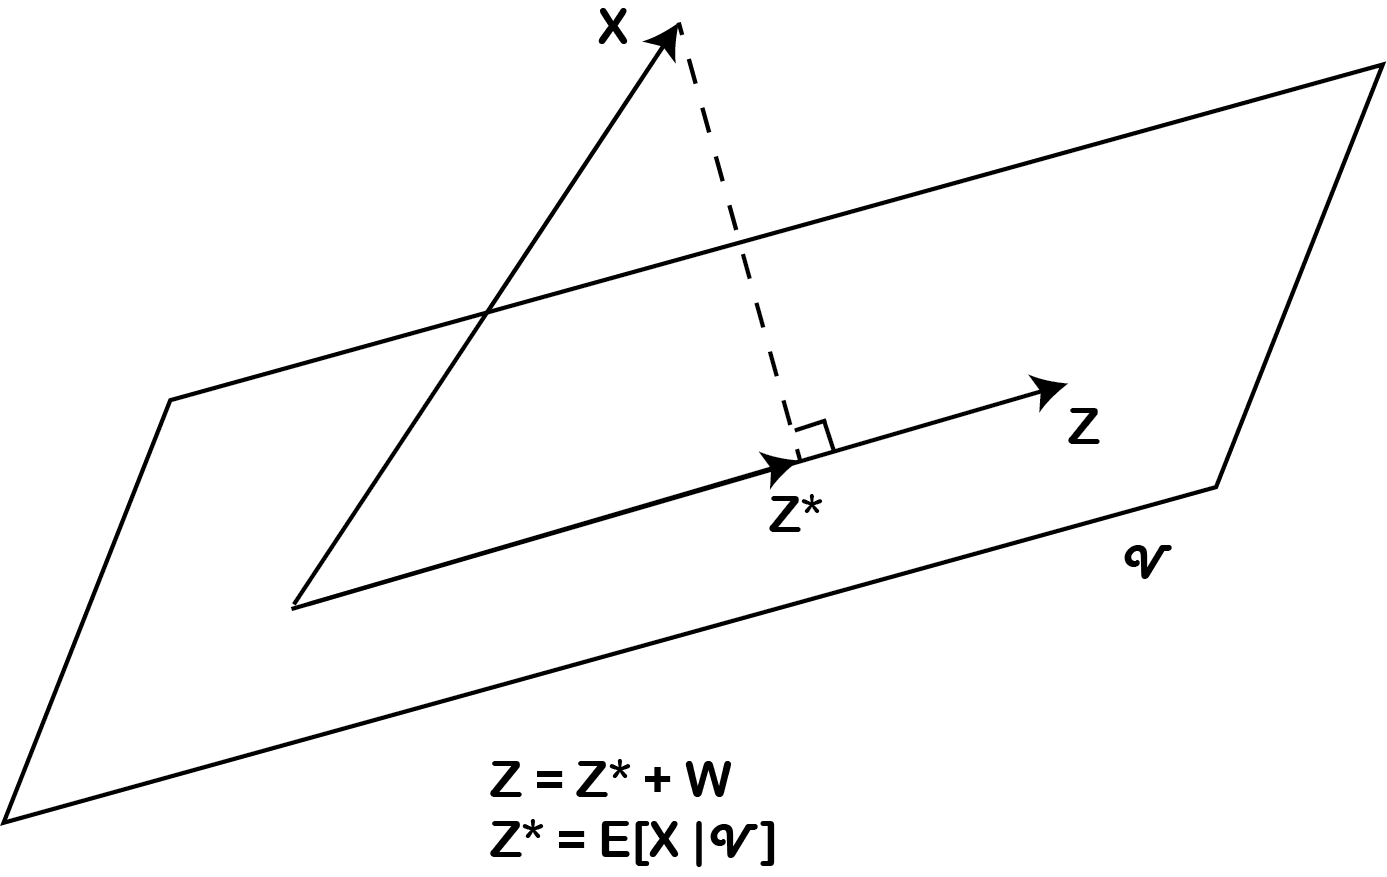
\includegraphics[width=0.4\textwidth]{figs/conditional_expectation.png}
\end{figure}
\end{frame}

\begin{frame}{Setting}
    Let $(\Omega,\mathcal F,\mathbb P)$ be a probability space and $L^2:=L^2(\Omega,\mathcal F,\mathbb P)$ with
    $\langle U,V\rangle=\mathbb E[UV]$.  
    Fix a sub-$\sigma$-field $\mathcal G\subset\mathcal F$ and denote the closed subspace
    \[
    \mathcal V:=L^2(\mathcal G)=\{Z\in L^2: Z \text{ is }\mathcal G\text{-measurable}\}.
    \]
    \textbf{Claim.} For $X\in L^2$,
    \[
    Z^*:=\mathbb E[X\mid\mathcal G]\in\mathcal V
    \quad\text{and}\quad
    Z^*=\arg\min_{Z\in\mathcal V}\ \mathbb E[(Z-X)^2].
    \]
    \end{frame}

    \begin{frame}{Proof of the claim}
    For any $Z\in\mathcal V$,
    \[
    \langle X-Z^*, Z\rangle
    =\mathbb E\!\left[(X-Z^*)Z\right]
    =\mathbb E\!\left(\mathbb E[(X-Z^*)Z\mid\mathcal G]\right)
    =\mathbb E\!\left(Z\,\mathbb E[X-Z^*\mid\mathcal G]\right)=0.
    \]
    Hence $X-Z^*\perp\mathcal V$.
    \vspace{1em}
 
    Let any $Z\in\mathcal V$ be written as $Z=Z^*+W$ with $W\in\mathcal V$. Then
    \[
    \|X-Z\|_2^2=\|X-(Z^*+W)\|_2^2
    =\|X-Z^*\|_2^2+\|W\|_2^2
    \ge \|X-Z^*\|_2^2,
    \]
    because $\langle X-Z^*,W\rangle=0$.  
    Equality $\Leftrightarrow W=0 \Leftrightarrow Z=Z^*$, proving uniqueness and the minimizer claim.
\end{frame}


\begin{frame}{Revisit several models}
\begin{enumerate}
    \item Score model 
    \begin{equation}
        Loss_{score} = \|s_\theta(\Tilde{x}) - \frac{\epsilon}{\sigma}\|^2;
    \end{equation}
    \item $X$ prediction model ( denoising model, $x0$ model)
    \begin{equation}
        Loss_{x_0} = \|x_\theta (\Tilde{x})-x\|^2,
    \end{equation}
    with 
    \begin{equation}
        s(\Tilde{x}) = -\frac{\Tilde{x}-\alpha x_{\theta^*} (\Tilde{x})}{\sigma^2}
    \end{equation}
    where $x_\theta(\Tilde{x}) \to x_{\theta^*}(\Tilde{x})\equiv \mathbb{E}[x|\Tilde{x}]$;
    \item $\epsilon$ prediction model
    \begin{equation}
        Loss_{\epsilon} = \|\epsilon_\theta(\Tilde{x})-\epsilon\|^2,
    \end{equation}
    with
    \begin{equation}
        s(\Tilde{x}) = -\frac{\epsilon_{\theta^*}(\Tilde{x})}{\sigma},
    \end{equation}
    where $\epsilon_\theta(\Tilde{x})\to\epsilon_{\theta^*}(\Tilde{x})\equiv\mathbb{E}[\epsilon|\Tilde{x}]$.
\end{enumerate}
\end{frame}

\begin{frame}{The consistency of the three modeling}

As stated before, we have the following connection in the optimal $(\theta^*)$ case
\begin{equation}
    s_{\theta^{*}}(\Tilde{x}) = -\frac{\Tilde{x}-\alpha x_{\theta^*} (\Tilde{x})}{\sigma^2} =  -\frac{\epsilon_{\theta^*}(\Tilde{x})}{\sigma},
\end{equation}
by the above conditional expectation. 

Hence, in the real modeling of designing the loss, we use the connection of three models without reaching the optimal parameter
\begin{equation}
    s_\theta(\Tilde{x}) = -\frac{\Tilde{x}-\alpha x_{\theta} (\Tilde{x})}{\sigma^2} =  -\frac{\epsilon_{\theta}(\Tilde{x})}{\sigma},
\end{equation}
and substitute each other form to the loss definition above, we can recover all of the losses given by different models.
\end{frame}


\section{Potential Score Matching loss}
% ============================================================
\begin{frame}{Key Identity: Jacobian Switch (chain rule between $\vx_0$ and $\vx_t$)}
    The Gaussian transition density is
    \[
    q(\vxt\mid \vxz) = \mathcal{N}\!\big(\vxt;\; \alpt\,\vxz,\, \sigt^2\mathbf{I}\big) \propto \exp\!\Big(-\tfrac{\|\vxt-\alpt\,\vxz\|^2}{2\sigt^2}\Big).
    \]
    A basic but crucial identity:
    \[
    \grad_{\vxt} q(\vxt\mid \vxz) = -\frac{1}{\alpt}\,\grad_{\vxz} q(\vxt\mid \vxz),\qquad (\alpt>0).
    \]
    \textbf{Proof sketch.} Differentiating the exponent w.r.t. \(\vxt\) and w.r.t. \(\vxz\) shows
    \(
    \grad_{\vxt}\!\|\vxt-\alpt\vxz\|^2 = 2(\vxt-\alpt\vxz),\;
    \grad_{\vxz}\!\|\vxt-\alpt\vxz\|^2 = -2\alpt(\vxt-\alpt\vxz),
    \)
    thus the factor $-1/\alpt$.
\end{frame}
    
    % ============================================================
    \begin{frame}{Theorem 1: Score as Conditional Force Expectation}
    \textbf{Statement.} With \(p(\vxz)\propto e^{-E(\vxz)/\kbT}\) and \(\vxt = \alpt\,\vxz+\sigt\,\veps\),
    \[
    \boxed{\;\grad_{\vxt}\log p(\vxt) 
    = \frac{1}{\alpt}\, \EE_{\vxz\mid \vxt}\Big[\frac{\vF(\vxz)}{\kbT}\Big]\;,}\qquad \vF(\vxz) = -\grad_{\vxz}E(\vxz).
    \]
    \textbf{Derivation.}
    \begin{align*}
    \grad_{\vxt}\log p(\vxt)
    &= \frac{\grad_{\vxt}\int p(\vxz)\, q(\vxt\mid\vxz)\,\dd \vxz}{p(\vxt)}\\
    &= \frac{1}{p(\vxt)}\int p(\vxz)\, \grad_{\vxt} q(\vxt\mid\vxz)\,\dd \vxz
    \end{align*}
\end{frame}

\begin{frame}{Theorem 1: Derivation (Cont)}
\begin{proofs}[\proofname\ (Cont)]
Using the Jacobian switch identity $(\ast)$:
\begin{align*}
    &\overset{(\ast)}{=} \frac{1}{p(\vxt)}\int p(\vxz)\,\Big(-\frac{1}{\alpt}\Big)\grad_{\vxz} q(\vxt\mid\vxz)\,\dd \vxz\\
    &= -\frac{1}{\alpt}\,\frac{1}{p(\vxt)}\int q(\vxt\mid\vxz)\, \grad_{\vxz} p(\vxz)\,\dd \vxz
\end{align*}
\end{proofs}
\end{frame}

\begin{frame}{Theorem 1: Derivation (Final)}
\begin{proofs}[\proofname\ (Cont)]
\begin{align*}
    &= -\frac{1}{\alpt}\int \underbrace{\frac{p(\vxz) q(\vxt\mid\vxz)}{p(\vxt)}}_{p(\vxz\mid\vxt)}\, \grad_{\vxz}\log p(\vxz)\,\dd \vxz\\
    &= \frac{1}{\alpt}\, \EE_{\vxz\mid\vxt}\Big[\frac{-\grad_{\vxz}E(\vxz)}{\kbT}\Big] 
    = \frac{1}{\alpt}\, \EE_{\vxz\mid\vxt}\Big[\frac{\vF(\vxz)}{\kbT}\Big]
\end{align*}
\end{proofs}
\end{frame}

\begin{frame}{Experiments on first 1, 000 frames for
    LJ data}
    \begin{figure}
        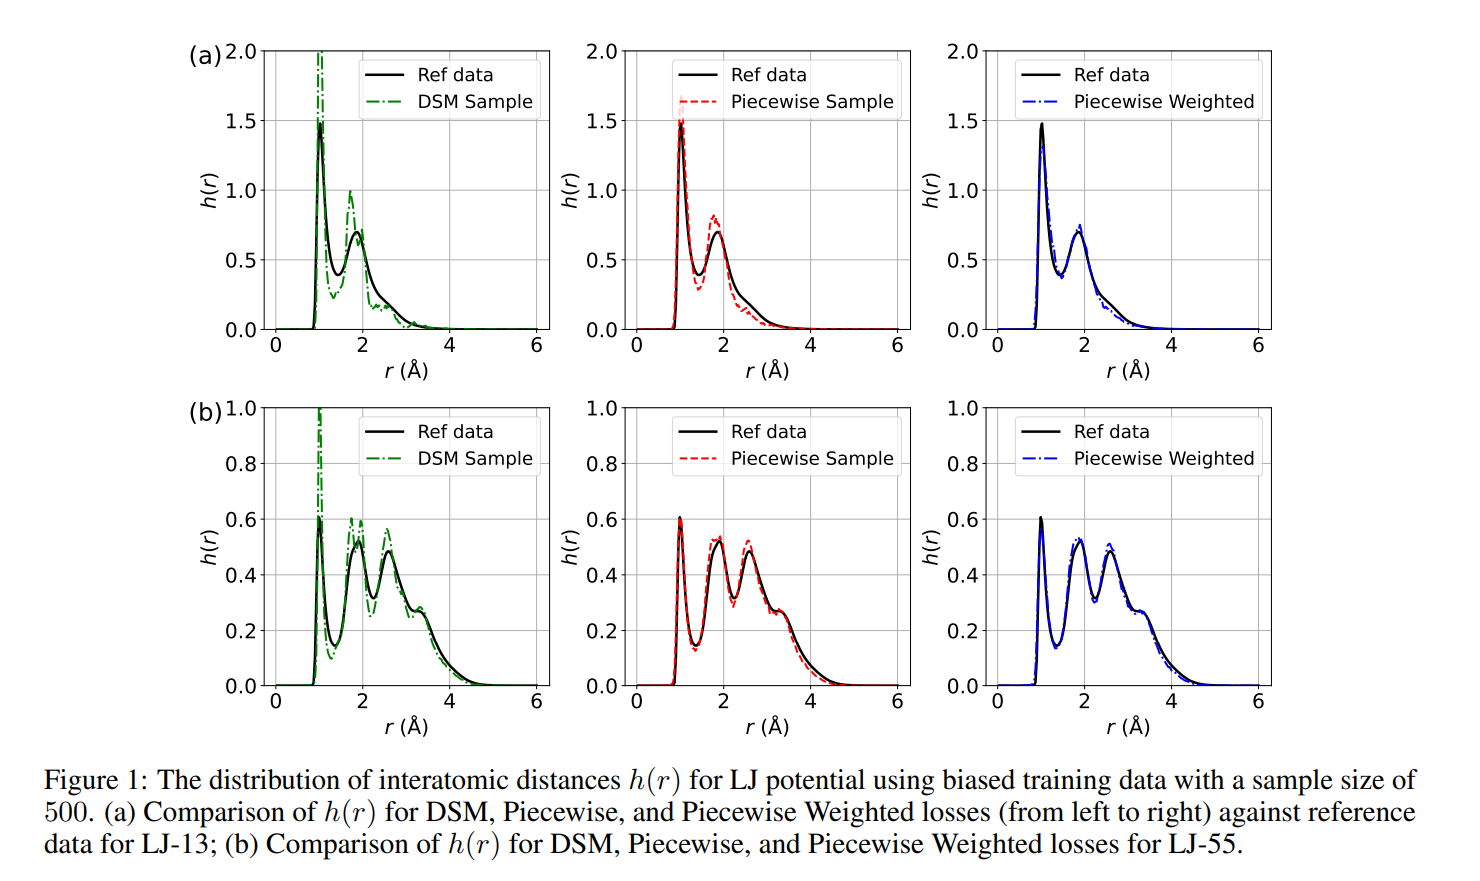
\includegraphics[width=0.8\textwidth]{figs/psm0.png}
    \end{figure}
\end{frame}

\begin{frame}{Experiments on first 5, 000 frames for MD reference trajectories}
    \begin{figure}
        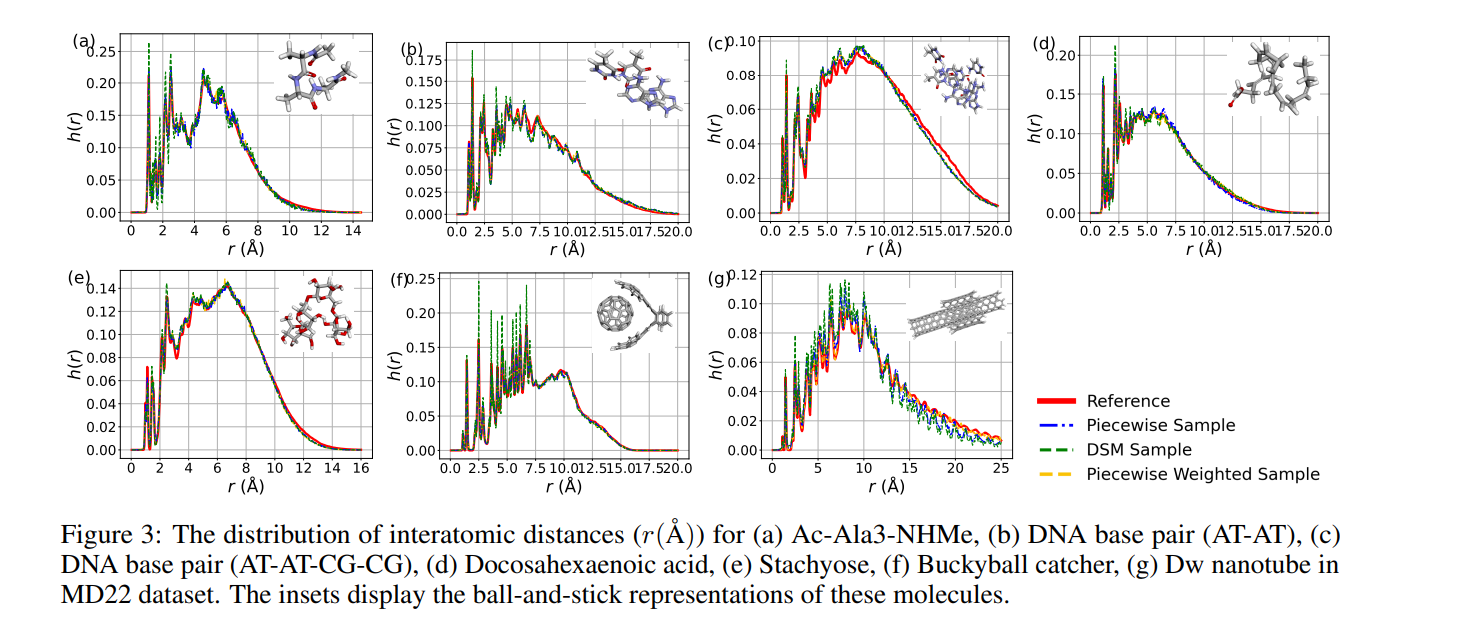
\includegraphics[width=0.9\textwidth]{figs/psm.png}
    \end{figure}
\end{frame}

\section{Diffusion model: from theories to implementation}
\begin{frame}{From Theory to Practice}
Now that we have established the theoretical foundations of score matching and diffusion processes, let's explore how these concepts are implemented in practice through several key approaches:

\begin{itemize}
    \item \textbf{SMLD} (Score Matching Langevin Dynamics)
    \item \textbf{DDPM} (Denoising Diffusion Probabilistic Models)  
    \item \textbf{Continuous formulations} and their advantages
\end{itemize}

Each approach offers different insights into the practical implementation of diffusion-based generative models.
\end{frame}

\begin{frame}{SMLD}
    Score Matching Langevin Dynamic (SMLD) (Song, 2019) adding noise in a following manner
    \begin{equation}
        p(\Tilde{x}_i| x) = N(\Tilde{x}_i; x, \sigma_i^2)\equiv Ce^{-\frac{\|\Tilde{x}_i-x\|^2}{2\sigma_i^2}},
    \end{equation}
    where a geometric sequence $\sigma_1> \sigma_2>\cdots > \sigma_T \approx
    0$ is given to add noise with different level.

    In a random variable view, 
    \begin{equation}
        \Tilde{x}_i = x + \sigma_i \epsilon
    \end{equation}
    for different $\sigma_i$ to get different noised random variable $\Tilde{x}_i$.

    Training object $J_{DSM}$ is given by 
    \begin{equation}
        J_{DSM} = \frac{1}{2}\mathbb{E}_{\sigma_i}\mathbb{E}_{p(x)}\mathbb{E}_{p(\Tilde{x}_i|x)}\left[\|s_\theta(\Tilde{x}_i,\sigma_i)+\frac{\Tilde{x}_i-x}{\sigma_i^2}\|^2\right].
    \end{equation}

    Anneled Langevin MCMC for sampling 
    \begin{equation}
        x_t = x_{t-1} + \frac{\Delta t}{2}S_\theta(x_{t-1}) + \sqrt{\Delta t}\epsilon, \quad \epsilon\sim N(0,1).
    \end{equation}
\end{frame}

\begin{frame}{DDPM}
    denoising diffusion probabilistic models (DDPM) (Ho, 2020) 
    \begin{enumerate}
        \item Derived from the Evidence Lower BOund (ELBO), \textcolor{red}{Not} score matching.
        \item First provide adding noise and denoise in the forward and reverse process. 
    \end{enumerate} 

The main procedure
\begin{enumerate}
    \item Adding noise 
    \begin{equation}
        x_t = \sqrt{1-\beta_t}x_{t-1} +\sqrt{\beta_t}\epsilon;
    \end{equation}
    \item Transition kernel 
    \begin{equation}
        p(x_t|x_0) = N(x_t;\alpha_t x_0, \sigma_t^2),
    \end{equation}
    where $\alpha_t = \prod_{i=1}^{t} \sqrt{1-\beta_i}$ and $\sigma_t^2 = 1-\alpha_t^2$.
\end{enumerate}
\end{frame}

\begin{frame}{DDPM}
The main procedure (Continued)
\begin{enumerate}
    \item Adding noise 
    \begin{equation}
        x_t = \sqrt{1-\beta_t}x_{t-1} +\sqrt{\beta_t}\epsilon;
    \end{equation}
    \item Transition kernel 
    \begin{equation}
        p(x_t|x_0) = N(x_t;\alpha_t x_0, \sigma_t^2), \text{ i.e., } x_t = \alpha_t x_0 + \sigma_t \epsilon,
    \end{equation}
    where $\alpha_t = \prod_{i=1}^{t} \sqrt{1-\beta_i}$ and $\sigma_t^2 = 1-\alpha_t^2$.
    \item Training Loss
    \begin{equation}
        \mathbb{E}_{t\sim U[0,1]}\mathbb{E}_{p(x)}\mathbb{E}_{p(x_t|x)}\left[\|\epsilon_\theta(x_t,t)-\epsilon\|^2\right],
    \end{equation}
    where we have used the approximation
        $x_0 = \frac{x_t-\sigma_t\epsilon}{\alpha_t}$.
    \\[-1em]
    \item Sampling 
    \begin{equation}
        x_{t-1} = \frac{1}{\sqrt{1-\beta_t}}(x_t+\beta_t s_\theta(x_t, t)) +\sqrt{\beta_t}\epsilon_t, \quad t = T, T-1, \cdots, 1.
    \end{equation}
\end{enumerate}
\end{frame}

\section{Continuous version of Diffusion Model}

\begin{frame}{The continuous version of SMLD}
Recall that
\begin{equation}
    x_t = x_0 + \sigma_t\epsilon,
\end{equation}
we can prove that 
\begin{equation}
    x_t = x_{t-1} + \sqrt{\sigma_t^2-\sigma_{t-1}^2}\epsilon.
\end{equation}
\begin{proof}
    We can prove the formula by a Recurrence 
    \begin{equation}
    \begin{aligned}
        x_t &= x_{t-1} + \sqrt{\sigma_t^2-\sigma_{t-1}^2}\epsilon\\
        & = x_{t-2} + \sqrt{\sigma_{t-1}^2-\sigma_{t-2}^2}\epsilon +\sqrt{\sigma_t^2-\sigma_{t-1}^2}\epsilon\\
        & = x_{t-2} + \sqrt{\sigma_t^2-\sigma_{t-2}^2}\epsilon\\
        & = ...= x_0 + \sigma_t\epsilon, \quad \text{ where } \sigma_0\approx 0.
    \end{aligned}
    \end{equation}
\end{proof}
\end{frame}

\begin{frame}{The continuous version of SMLD}
From 
\begin{equation}
    x_t = x_{t-1} + \sqrt{\sigma_t^2-\sigma_{t-1}^2}\epsilon,
\end{equation}
we have 
\begin{equation}
    \begin{aligned}
        \Delta x_t &= \sqrt{\frac{\sigma_t^2-\sigma_{t-1}^2}{\Delta t}}\sqrt{\Delta t}\epsilon\\
        &= \sqrt{\frac{\sigma_t^2-\sigma_{t-1}^2}{\Delta t}}\Delta B_t.
    \end{aligned}
\end{equation}
Further, let $\Delta t\to 0$, we have
\begin{equation}
    dx = \sqrt{\frac{d\sigma_t^2}{d t}}dB_t.
\end{equation}
\end{frame}

\begin{frame}{The continuous version of DDPM}
Recall that 
\begin{equation}
        x_t = \sqrt{1-\beta_t}x_{t-1} +\sqrt{\beta_t}\epsilon.
\end{equation}
Similarly 
\begin{equation}
    \begin{aligned}
        x_t\approx (1-\frac{1}{2}\beta_t)x_{t-1} + \sqrt{\beta_t}\epsilon,
    \end{aligned}
\end{equation}
hence, we have
\begin{equation}
    \begin{aligned}
        \Delta x_t &= -\frac{1}{2}\Tilde{\beta_t} x_{t-1}\Delta t + \sqrt{\Tilde{\beta_t}}\sqrt{\Delta t}\epsilon, \quad \text{ where } \Tilde{\beta_t} = \frac{\beta_i}{\Delta t}\\
        & = -\frac{1}{2}\Tilde{\beta_t} x_{t-1}\Delta t + \sqrt{\Tilde{\beta_t}}\Delta B_t.
    \end{aligned}
\end{equation}
Further, let $\Delta t\to 0$, we finally obtain
\begin{equation}
    dx = -\frac{1}{2}\Tilde{\beta_t} x d t + \sqrt{\Tilde{\beta_t}}d B_t.
\end{equation}
\end{frame}

\begin{frame}{VE \& VP}
Summarizing the form of continuous DDPM and SMLD, we summarize the adding noise process as
\begin{equation}\label{eq:forward}
    dx = f(x, t)dt + g(t) dB_t,
\end{equation}
where the corresponding distribution $p(x, t)$ satisfying the following Fokker-Planck equation
\begin{equation}\label{eq:fp}
    \frac{\partial p(x,t)}{\partial t} + \nabla\cdot\left(f(x,t) p(x,t)\right) -\frac{1}{2}g^2(t) \triangle p(x,t)=0.
\end{equation}

Training DSM object 
\begin{equation}
    J_{DSM} = \mathbb{E}_{t\sim U[0,1]}\mathbb{E}_{p(x_0)}\mathbb{E}_{p(x_t|x_0)}\left[\|s_\theta(x_t,t)-\textcolor{red}{\nabla_{x_t}\log p(x_t|x_0)}\|^2\right].
\end{equation}
\end{frame}


\begin{frame}{VE \& VP adding noise}
To training the Denoising Score Match loss $J_{DSM}$ above, the key is to add noise by the transition kernel
\begin{equation}
    p(\Tilde{x}|x) \equiv p(x(t)|x(0)) = N(x(t); \Tilde{\alpha}_t x(0), \Tilde{\sigma}_t^2),
\end{equation}
from which we can obtain the noised data 
\begin{equation}
    x(t) = \Tilde{\alpha}_t x(0) + \Tilde{\sigma}_t\epsilon, \quad \epsilon\sim N(0,1).
\end{equation}

\textcolor{red}{The question becomes}: Given VE \& VP 
\begin{equation}
    dx = \sqrt{\frac{d[\sigma^2]}{dt}} dB_t,\quad 
    dx = -\frac{1}{2}\Tilde{\beta_t} x d t + \sqrt{\Tilde{\beta_t}}d B_t.
\end{equation}
how to derive $p(x(t)|x(0))$, i.e., $p(\Tilde{x}|x)$ for adding noise?
\end{frame}

\begin{frame}{VE \& VP Transition kernel}
The summarizing form of VE \& VP is 
\begin{equation}
    dx = h(t)xdt+ g(t)dB_t,
\end{equation}
where $h(t)=0$ for VE and $h(t)=-\frac{1}{2}\Tilde{\beta}(t)$ for VP. 

\begin{lemma}
Let $\mu(t) =\mathbb{E}[x(t)]$ and $\Sigma(t)=\mathbb{E}\left[(x-\mu(t))(x-\mu(t))^T\right]$, we have the following formula
\begin{equation}
\begin{aligned}
    \frac{d\mu(t)}{dt} = h(t)\mu(t),\quad
    \frac{d\Sigma(t)}{dt} = 2h(t)\Sigma(t)+g^2(t)I.
\end{aligned} 
\end{equation}
\end{lemma}
The proof of the Lemma can be found in a stochastic differential equation textbook such as Applied Stochastic Differential Equations, S\"{a}rkk\"{a} and Solin, 2019.
\end{frame}

\begin{frame}{VE \& VP Transition kernel}

\begin{lemma}
    For VE, the transition kernel is given by the following formula
\begin{equation}\label{eq:tranve}
    P(x(t)|x(0)) = N(x(t); x(0), \sigma^2(t)-\sigma^2(0)).
\end{equation}
For VE, 
\begin{equation}
    \Tilde{\alpha}_t \equiv  1, \quad \Tilde{\sigma}^2_t \equiv \sigma^2(t)-\sigma^2(0)\approx \sigma^2(t).
\end{equation}
\end{lemma}

\begin{lemma}
    For VP, the transition kernel is given the following formula
\begin{equation}\label{eq:tranvp}
    p(x(t)|x(0)) = N\left(x(t); x(0)e^{-\frac{1}{2}\int_0^t \Tilde{\beta}(s)ds},1-e^{-\int_0^t \Tilde{\beta}(s)ds}\right).
\end{equation}
For VP, 
\begin{equation}
    \Tilde{\alpha}_t \equiv  e^{-\frac{1}{2}\int_0^t \Tilde{\beta}(s)ds}, \quad \Tilde{\sigma}^2_t \equiv 1-e^{-\int_0^t \Tilde{\beta}(s)ds}.
\end{equation}
\end{lemma}
\end{frame}


\begin{frame}{Proof of VE transition kernel}
\begin{proof}
For VE, by a simple calculation we have

\begin{equation}
        \frac{d\mu(t)}{dt} = 0,\quad \frac{d\Sigma(t)}{dt} = \frac{d[\sigma^2(t)]}{dt},
\end{equation}
Hence, it is easy to obtain the following form 
\begin{equation}
        \mu(t) = \mu(0) = x(0),\quad \Sigma(t) = \sigma^2(t)-\sigma^2(0).
\end{equation}
Here we have used the fact  
\begin{equation}
    \mu(0) = x(0), \quad \Sigma(0)=0
\end{equation}
as $x(0)$ is taken as a constant, not a random variable.
And we obtain 
\begin{equation}
    P(x(t)|x(0)) = N(x(t); x(0), \sigma^2(t)-\sigma^2(0)).
\end{equation}
\end{proof}
\end{frame}

\begin{frame}{VP Proof: Differential Equations}
\begin{proof}
For VP, we have the differential equations:
\begin{equation}
    \frac{d\mu(t)}{dt} = -\frac{1}{2}\beta(t)\mu(t)
\end{equation}
\begin{equation}
    \frac{d\Sigma(t)}{dt} = -\beta(t)\Sigma(t)+\beta(t)
\end{equation}
We solve these using integrating factors.
\end{proof}
\end{frame}

\begin{frame}{VP Proof: Integrating Factors}
\begin{proofs}[\proofname\ (Cont)]
For the mean equation, multiply by $e^{\int_0^t\frac{1}{2}\beta(s)ds}$:
\begin{equation}
    \frac{d\mu(t)}{dt}e^{\int_0^t\frac{1}{2}\beta(s)ds} + \frac{1}{2}\beta(t)\mu(t) e^{\int_0^t\frac{1}{2}\beta(s)ds} =0
\end{equation}
For the variance equation, multiply by $e^{\int_0^t\beta(s)ds}$:
\begin{equation}
    \frac{d\Sigma(t)}{dt}e^{\int_0^t\beta(s)ds} +\beta(t)\Sigma(t)e^{\int_0^t\beta(s)ds} = \beta(t)e^{\int_0^t\beta(s)ds}
\end{equation}
\end{proofs}
\end{frame}

\begin{frame}{VP Proof: Solution}
\begin{proofs}[\proofname\ (Cont)]
This gives us:
\begin{equation}
    \frac{d}{dt} (\mu(t)e^{\int_0^t\frac{1}{2}\beta(s)ds}) = 0
\end{equation}
\begin{equation}
    \frac{d}{dt} (\Sigma(t)e^{\int_0^t\beta(s)ds}) = \frac{d}{dt} e^{\int_0^t\beta(s)ds}
\end{equation}
Solving with initial conditions $\mu(0) = x(0)$, $\Sigma(0) = 0$:
\begin{equation}
    p(x(t)|x(0)) = N\left(x(t); x(0)e^{-\frac{1}{2}\int_0^t \beta(s)ds},1-e^{-\int_0^t \beta(s)ds}\right)
\end{equation}
\end{proofs}
\end{frame}

\begin{frame}{Revisit adding noise}
The \textbf{equivalence} of the adding noise
\begin{enumerate}
    \item From the stochastic process, denote the variable $x_t$, we have 
    \begin{equation}
        d x_t = f(x,t)dt + g(t)dB_t, 
    \end{equation}
    with corresponding discrete form (Euler-Maruyama scheme)
    \begin{equation}
        x_{t+\Delta t} = x_{t} + f(x_t, t)\Delta t + g(t)\sqrt{\Delta t}\epsilon, \quad \epsilon\sim N(0, 1). 
    \end{equation}
\item From transition kernel perspective, 
\begin{equation}
    p(x_t) = \int_{x_0} p(x_0)p(x_t|x_0)dx_0,
\end{equation}
where 
\begin{equation}
    p(x_t|x_0) = N(x_t; \mu_t, \Sigma_t)=N(x_t; \Tilde{\alpha}_tx_0, \Tilde{\sigma}_t^2)=\frac{1}{C}e^{-\frac{\|x_t-\mu_t\|^2}{2\Sigma_t}}.
\end{equation}
\end{enumerate}

\end{frame}

\begin{frame}{Training recipe}
The training for VE follows the following process (VP is in a similar way)
\begin{enumerate}
    \item Random choose one data $x\sim p_{data}$;
    \item Random sample $t\sim U[0, 1]$;
    \item Random sample a white noise $\epsilon\sim N(0, 1)$;
    \item Adding noise 
    \begin{equation}
        x_t = \Tilde{\alpha}_t x + \Tilde{\sigma}_t\epsilon, 
    \end{equation}
    where the mean value $\Tilde{\alpha}_t x= x(0)$  and standard deviation $\Tilde{\sigma}_t = \sqrt{\sigma^2(t)-\sigma^2(0)}\approx \sigma(t)$ in VE referring to \eqref{eq:tranve}. VP is similar with the mean and standard deviation from its transition kernel \eqref{eq:tranvp};
    \item Compute the Loss
    by summation the following norm over $x$, $t$ and $\epsilon$ 
    \begin{equation}  
    \|s_\theta(x_t, t)-\epsilon/\Tilde{\sigma}_t\|.
    \end{equation} 
\end{enumerate}
\end{frame}


\begin{frame}{Inference: Reverse denoising process}
The reverse denoising process is given by 
\begin{equation}\label{eq:reverse}
    dx = (f(x,t)-g^2\nabla_x \log p(x,t))dt + g(t)dB_t,
\end{equation}
or 
\begin{equation}
    dx = (f(x,t)-\frac{1}{2}g^2\nabla_x \log p(x,t))dt,
\end{equation}
or 
\begin{equation}\label{eq:reverse2}
    dx = (f(x,t)-\frac{3}{2}g^2\nabla_x \log p(x,t))dt + \sqrt{2}g(t)dB_t,
\end{equation}
\begin{equation}
    \cdots
\end{equation}
Due to obeying the same Fokker-Planck equation for $p(x, t)$
\begin{equation}
    \frac{\partial p(x,t)}{\partial t} + \nabla\cdot(f(x,t) p(x,t)) -\frac{1}{2}g^2(t) \triangle p(x,t)=0.
\end{equation}
\end{frame}

\begin{frame}{Reverse Process Proof: Setup}
We prove the first reverse sampling form \eqref{eq:reverse}. The Fokker-Planck equation of the forward process \eqref{eq:forward} is:
\begin{equation}
    \frac{\partial p}{\partial t} + \nabla \cdot (f(x,t)p)-\frac{1}{2}g^2\triangle p = 0.
\end{equation}
Let $t = T-\tau$, we have:
\begin{equation}
    \frac{\partial p}{\partial \tau} - \nabla\cdot (f(x,T-\tau) p) + g^2\triangle p -\frac{1}{2}g^2\triangle p =0.
\end{equation}
\end{frame}

\begin{frame}{Reverse Process Proof: Derivation}
\begin{proofs}[\proofname\ (Cont)]
By $\nabla\cdot\nabla = \triangle$ and $\nabla \log p=\nabla p/p$:
\begin{equation}
    \frac{\partial p}{\partial \tau} - \nabla\cdot \bigg(\left(f(x,T-\tau)-g^2\nabla\log p\right)p\bigg) -\frac{1}{2}g^2\triangle p =0.
\end{equation}
Hence, we obtain the corresponding SDE form:
\begin{equation}
    dx = -(f(x, T-\tau)-g^2\nabla\log p)d\tau + gdB_\tau
\end{equation}
By substitution $\tau = T-t$:
\begin{equation}
    dx = (f(x,t)-g^2\nabla\log p)dt + gdB_t
\end{equation}
\end{proofs}
\end{frame}

% \begin{frame}{Interesting property about the ODE and SDE}
% \begin{enumerate}
%     \item The forward SDE and the reverse SDE has different sign 
% \end{enumerate}
% \end{frame}

\begin{frame}{Inference recipe}
The inference for VE follows the following process (VP is in a similar way)
\begin{enumerate}
    \item Random generate a noise at time $t=1$ as $x(1)\sim N(0, \sigma^2_{max})$;
    \item Integrate the reverse sampling equation 
    \begin{equation}
        dx = \left(f(x,t)-g^2(t) s_\theta(x,t)\right)dt + g(t)dB_t
    \end{equation} or 
    \begin{equation}
        dx = (f-\frac{1}{2}g^2 s_\theta)dt
    \end{equation}
    over the time span $[0, 1]$ to get $x(0)$.
    \item Corrector process: at each internal value $x(t)$, we can relax the value $x(t)$ by a corrector, which takes the Langevin MCMC process. 
\end{enumerate}

\end{frame}


\begin{frame}{The Corrector: revisit Langevin MCMC}
The Langevin diffusion process is given by 
\begin{equation}
    x_i = x_{i-1}+\frac{\Delta t}{2}\textcolor{red}{\nabla_x\log p(x_{i-1})}+\sqrt{\Delta t}\epsilon, \quad \epsilon\sim N(0, 1).
\end{equation}
We can prove   $\pi(x)$ of the obtained data points $\{x_i\}_{i=1}^N$ converges to $p(x)$.

\begin{proofs}
The continuous form of the scheme is:
\begin{equation}
    dx = \frac{1}{2}\nabla\log p(x) dt + dB_t.
\end{equation}
The corresponding Fokker-Planck equation is:
\begin{equation}
\frac{\partial\pi(x,t)}{\partial t} + \nabla\cdot(\frac{1}{2}\nabla\log p(x) \pi(x,t)) -\frac{1}{2}\triangle \pi(x,t) = 0.
\end{equation}
With sufficient time evolution, the distribution converges to a stable distribution where:
\begin{equation}
    \frac{\partial \pi(x,t)}{\partial t} = 0, \quad t\to \infty.
\end{equation}
\end{proofs}
\end{frame}

\begin{frame}{The Corrector: revisit Langevin MCMC}

\begin{proofs}[\proofname\ (Cont)]
Hence we have:
\begin{equation}
    \nabla\cdot(\pi\nabla\log p - \nabla\pi) = 0, \quad \forall x.
\end{equation}
Therefore:
\begin{equation}
    \nabla\log p = \nabla\log \pi
\end{equation}
given that $\pi>0$ almost everywhere. 
Hence:
\begin{equation}
    \pi^*(x) = p(x)
\end{equation}
where $\pi^*$ is the stable distribution of $\pi(x, t)$.
\end{proofs}
\end{frame}

\section{More papers}
\begin{frame}{Additional Important Papers}
The field of diffusion models has evolved rapidly with many important contributions. Here we highlight several key papers that have shaped the current understanding and practice:

\begin{itemize}
    \item \textbf{DDPM} - The foundational work on denoising diffusion probabilistic models
    \item \textbf{EDM} - Elucidating design choices for better performance
    \item \textbf{DPM-Solver} - Fast ODE solvers for efficient sampling
    \item \textbf{Consistency Models} - One-step generation with diffusion quality
\end{itemize}

These papers represent significant advances in making diffusion models more practical and efficient.
\end{frame}

\subsection{DDPM: Denoising Diffusion Probabilistic Models}
\begin{frame}{DDPM: Goal \& Setup}
\textbf{Goal.} Learn a generative model $p_\theta(x_0)$ by reversing a noisy diffusion.\\[4pt]
\textbf{Latents.} Introduce $x_{1:T}$ with same dimensionality as data $x_0$.\\[4pt]
\textbf{Reverse (sampling) chain:}
\[
p_\theta(x_{0:T}) = p(x_T)\prod_{t=1}^{T} p_\theta(x_{t-1}\mid x_t),\quad
p(x_T)=\mathcal N(0,I),
\]
\[
p_\theta(x_{t-1}\mid x_t)=\mathcal N\!\big(\mu_\theta(x_t,t),\,\Sigma_\theta(x_t,t)\big).
\]
\textbf{Forward (fixed) diffusion:}
\[
q(x_{1:T}\mid x_0)=\prod_{t=1}^{T} q(x_t\mid x_{t-1}),\quad
q(x_t\mid x_{t-1})=\mathcal N\!\big(\sqrt{1-\beta_t}\,x_{t-1},\,\beta_t I\big).
\]
With $\alpha_t:=1-\beta_t,\;\bar\alpha_t:=\prod_{s=1}^t\alpha_s$:
\[
q(x_t\mid x_0)=\mathcal N\!\big(\sqrt{\bar\alpha_t}\,x_0,\,(1-\bar\alpha_t)I\big).
\]
\end{frame}

\begin{frame}{DDPM: Training Objective (Variational Bound)}
Optimize the NLL via a reduced-variance ELBO:
\[
\mathbb E[-\log p_\theta(x_0)] \;\le\; 
\underbrace{\mathbb E\big[\mathrm{KL}(q(x_T|x_0)\,\|\,p(x_T))\big]}_{L_T}
+ \sum_{t=2}^{T} \underbrace{\mathbb E\big[\mathrm{KL}(q(x_{t-1}|x_t,x_0)\,\|\,p_\theta(x_{t-1}|x_t))\big]}_{L_{t-1}}
- \underbrace{\mathbb E[\log p_\theta(x_0|x_1)]}_{L_0}.
\]
Here $q(x_{t-1}\!\mid x_t,x_0)$ is Gaussian in closed form, so each KL has a tractable expression.\\[6pt]
\textbf{Data scaling.} Images scaled to $[-1,1]$; $p_\theta(x_0\!\mid x_1)$ is a discretized Gaussian decoder for likelihood evaluation.
\end{frame}

\begin{frame}{DDPM: $\epsilon$-Prediction Parameterization}
Write the forward noising as
\[
x_t = \sqrt{\bar\alpha_t}\,x_0 + \sqrt{1-\bar\alpha_t}\,\varepsilon,\quad \varepsilon\sim\mathcal N(0,I).
\]
Parameterize the reverse mean via a network $\varepsilon_\theta(x_t,t)$:
\[
\mu_\theta(x_t,t) \;=\; \frac{1}{\sqrt{\alpha_t}}\!\left(
x_t - \frac{1-\alpha_t}{\sqrt{\,1-\bar\alpha_t\,}}\;\varepsilon_\theta(x_t,t)\right).
\]
\textbf{Sampling step} (with fixed $\sigma_t$ such as $\sigma_t^2=\beta_t$ or $\tilde\beta_t$):
\[
x_{t-1} \;=\; \mu_\theta(x_t,t) \;+\; \sigma_t\,z,\quad z\sim\mathcal N(0,I).
\]
This connects DDPM to denoising score matching and (annealed) Langevin-like sampling.
\end{frame}

\begin{frame}{DDPM: Simplified Loss \& Algorithms}
\textbf{Simplified objective (``$L_{\text{simple}}$''):}
\[
\boxed{~~
\mathcal L_{\text{simple}}(\theta) \;=\; \mathbb E_{t\sim\mathcal U[1,T],\,x_0,\,\varepsilon}
\big\|\,\varepsilon - \varepsilon_\theta\!\big(\sqrt{\bar\alpha_t}\,x_0 + \sqrt{1-\bar\alpha_t}\,\varepsilon,\,t\big)\big\|_2^2
~~}
\]
\textbf{Training (sketch).}
\begin{enumerate}
  \item Sample $x_0\!\sim q(x_0),\; t\!\sim\!\mathrm{Unif}\{1,\ldots,T\},\; \varepsilon\!\sim\!\mathcal N(0,I)$.
  \item Form $x_t$ via the forward formula; take a GD step on $\|\varepsilon-\varepsilon_\theta(x_t,t)\|^2$.
\end{enumerate}
\textbf{Sampling (sketch).}
\begin{enumerate}
  \item $x_T\!\sim\!\mathcal N(0,I)$.
  \item For $t=T,\ldots,1$: compute $\mu_\theta(x_t,t)$, add noise $\sigma_t z$ if $t>1$ to get $x_{t-1}$.
\end{enumerate}
Empirically, $L_{\text{simple}}$ gives best sample quality; ELBO training gives better likelihoods.
\end{frame}

\begin{frame}{DDPM: Schedules, Architecture, \& Practice}
\textbf{Noise schedule.} Typical: $T{=}1000$, linear $\beta_t$ from $10^{-4}$ to $2{\times}10^{-2}$ (on $[-1,1]$ data); small $\beta_t$ keeps forward and reverse both Gaussian-friendly.\\[6pt]
\textbf{Network.} U-Net backbone (PixelCNN++-style), group norm, sinusoidal time embedding, self-attention at medium resolution (e.g., $16{\times}16$).\\[6pt]
\textbf{Tips.}
\begin{itemize}
  \item Fixed $\Sigma_\theta$ (e.g., $\sigma_t^2=\beta_t$ or $\tilde\beta_t$) stabilizes training.
  \item Dropout (small) on CIFAR-10 helps; EMA on params (e.g., 0.9999).
  \item Evaluate with FID/IS; likelihood via discretized decoder.
\end{itemize}
\end{frame}

\begin{frame}{DDPM: Intuitions \& Connections}
\textbf{Progressive generation.} Coarse structure emerges early (large $t$), details refine as $t\!\downarrow$.\\[4pt]
\textbf{Score-based view.} $\varepsilon_\theta$ learns noise (scaled score), making the sampler resemble annealed Langevin dynamics.\\[4pt]
\textbf{Autoregressive link.} The ELBO can be seen as progressive decoding with a generalized ``bit ordering.''\\[6pt]
\textbf{Why DDPM?}
\begin{itemize}
  \item High sample quality; stable training; flexible architectures.
  \item Trade-off: exact likelihoods lag some likelihood-based models, but samples excel.
\end{itemize}
\end{frame}

\subsection{EDM: Elucidating the Design Space of Diffusion-Based Generative Models
}

\begin{frame}{Big Picture}
\begin{itemize}
  \item Goal: separate \textbf{design choices} (sampling, schedules, preconditioning, training) to simplify and speed up diffusion models.
  \item Key outcomes:
    \begin{itemize}
      \item \textbf{Faster sampling} (tens of NFEs) with strong FID.
      \item Modular choices: ODE view, schedule $\sigma(t)$, scaling $s(t)$, time steps $\{t_i\}$, preconditioning, loss weighting.
    \end{itemize}
  \item Works as a \textbf{drop-in} improvement over prior models (VP/VE/DDIM/ADM).
\end{itemize}
\end{frame}

\begin{frame}{Common ODE Framework}
\textbf{Probability flow ODE} with schedule $\sigma(t)$ and (optional) scaling $s(t)$:
\[
\frac{d\bm{x}}{dt}
=
\Big(\frac{\dot{\sigma}}{\sigma} + \frac{\dot{s}}{s}\Big)\bm{x}
\;-\;
\frac{\dot{\sigma}\, s}{\sigma}\,\nabla_{\bm{x}}\log p\!\left(\tfrac{\bm{x}}{s};\sigma\right)
\]
Using denoising score matching,
\[
\nabla_{\bm{x}}\log p(\bm{x};\sigma)=\frac{D(\bm{x};\sigma)-\bm{x}}{\sigma^{2}},
\]
so the ODE is solved numerically by evaluating a \textbf{denoiser} $D_\theta(\bm{x};\sigma)$.
\medskip

\textbf{EDM choice:} set $\sigma(t)=t,\; s(t)=1$ $\Rightarrow$ straight(er) trajectories, stable integration.
\end{frame}

\begin{frame}{Denoising Score Matching (Training Target)}
Given clean $\bm{y}\!\sim\!p_{\text{data}}$, noise $\bm{n}\!\sim\!\mathcal{N}(0,\sigma^2 I)$,
\[
D(\bm{y}+\bm{n};\sigma)
\;=\;
\arg\min_{D}\,\mathbb{E}\,\|\;D(\bm{y}+\bm{n};\sigma)-\bm{y}\;\|_2^2,
\]
and
\[
\nabla_{\bm{x}}\log p(\bm{x};\sigma)=\frac{D(\bm{x};\sigma)-\bm{x}}{\sigma^2}.
\]
Train $D_\theta$ over a range of $\sigma$ to match the optimal denoiser; use it at test time to integrate the ODE.
\end{frame}


\begin{frame}{Fast Deterministic Sampling}
\textbf{Integrator:} Heun’s 2nd order (improved Euler) for better truncation error vs. Euler.
\[
\text{Predict: }\;\bm{x}_{i+1}^{(E)}=\bm{x}_i + \Delta t_i\, f(t_i,\bm{x}_i)
\quad
\text{Correct: }\;\bm{x}_{i+1}=\bm{x}_i + \Delta t_i\,
\frac{f(t_i,\bm{x}_i) + f(t_{i+1},\bm{x}_{i+1}^{(E)})}{2}
\]
\textbf{Noise levels / time steps:}
\[
\sigma_i
=
\Big(\sigma_{\max}^{1/\rho} + \tfrac{i}{N-1}\big(\sigma_{\min}^{1/\rho}-\sigma_{\max}^{1/\rho}\big)\Big)^{\rho},
\quad
t_i=\sigma_i,\quad \rho\approx 7.
\]
\textbf{Effect:} reach strong FID with far fewer NFEs (e.g., \(\sim\)35 for CIFAR-10).
\end{frame}

%------------------------------------------------------------
\begin{frame}{Stochastic Sampling (``Churn'')}
At step $i$ (noise $t_i$), temporarily \textbf{increase} noise:
\[
\hat{t}_i = t_i(1+\gamma_i), \quad \hat{\bm{x}}_i = \bm{x}_i + \sqrt{\hat{t}_i^2 - t_i^2}\;\bm{\varepsilon},\; \bm{\varepsilon}\sim\mathcal{N}(0,S_{\text{noise}}^2 I),
\]
then \textbf{one Heun step} from $\hat{t}_i$ to $t_{i+1}$ using $D_\theta$ evaluated at the \emph{post-churn} state $(\hat{\bm{x}}_i,\hat{t}_i)$.
\medskip

\textbf{Heuristics:}
\begin{itemize}
  \item Apply churn only for $t_i\!\in\![t_{\min}^{\star},t_{\max}^{\star}]$; set $\gamma_i\!=\!\text{Schurn}/N$, clamp to avoid excessive re-noising.
  \item Slightly inflate $S_{\text{noise}}\!>\!1$ to counter over-denoising bias.
\end{itemize}
\textbf{Use:} helpful on more diverse data; may be unnecessary (even harmful) once training is improved.
\end{frame}

\begin{frame}{Network Preconditioning}
Represent denoiser with \textbf{preconditioned} skip connection:
\[
D_\theta(\bm{x};\sigma)
=
c_{\text{skip}}(\sigma)\,\bm{x}
\;+\;
c_{\text{out}}(\sigma)\,F_\theta\!\big(c_{\text{in}}(\sigma)\,\bm{x};\;c_{\text{noise}}(\sigma)\big),
\]
Design $c_{\text{in}},c_{\text{out}},c_{\text{skip}}$ so that:
\begin{itemize}
  \item inputs/targets have \textbf{nearly unit variance} across $\sigma$,
  \item network errors are not \textbf{amplified} at large $\sigma$ (robust gradients),
  \item $F_\theta$ smoothly interpolates between predicting signal vs. noise.
\end{itemize}
This stabilizes training and unlocks better loss scheduling.
\end{frame}

\begin{frame}{Loss Weighting \& Noise-Level Sampling}
With the preconditioned form, the effective per-sample weight scales with $c_{\text{out}}(\sigma)^2$.
\[
\textbf{Set}\quad \lambda(\sigma)=\frac{1}{c_{\text{out}}(\sigma)^2}
\quad\Rightarrow\quad
\text{balanced contributions over }\sigma.
\]
Sample noise levels $\sigma$ from a \textbf{log-normal} (or similar) that prioritizes the \emph{perceptually relevant} mid-$\sigma$ range:
\[
\ln\sigma \sim \mathcal{N}(P_{\text{mean}},P_{\text{std}}^2).
\]
Result: large FID gains across datasets when combined with preconditioning.
\end{frame}

\begin{frame}{Augmentation Regularization (Non-Leaky)}
\begin{itemize}
  \item Apply standard geometric augmentations to training images \emph{before} adding noise.
  \item Feed augmentation parameters as conditioning to $F_\theta$ (\emph{non-leaky}); set to zero at inference.
  \item Helps small/medium datasets reduce overfitting; further FID improvements.
\end{itemize}
\end{frame}

\begin{frame}{Headline Results \& Takeaways}
\begin{itemize}
  \item \textbf{Sampling:} Heun(2) + $\sigma(t)\!=\!t$ + $\rho$-scheduled steps $\Rightarrow$ big NFE cuts at equal FID.
  \item \textbf{Training:} preconditioning + balanced loss + noise-level prior $\Rightarrow$ strong, robust models.
  \item \textbf{Stochasticity:} beneficial on harder data; unnecessary with strong training on simpler data.
  \item \textbf{Outcomes:} new SOTA-level FIDs on CIFAR-10 / ImageNet-64 with \textbf{much faster} sampling.
\end{itemize}
\end{frame}

\subsection{DPM-Solver: A Fast ODE Solver for Diffusion Probabilistic Models}

\begin{frame}{DPM-Solver: Motivation}
\begin{itemize}
  \item Diffusion models (DPMs) produce strong samples but are slow: \textbf{hundreds--thousands} of NFE.
  \item Sampling can be recast as solving a \textbf{probability flow ODE}: no stochasticity $\Rightarrow$ larger steps possible.
  \item \textbf{DPM-Solver} exploits the \emph{semi-linear} structure of the diffusion ODE to deliver high-quality samples in \textbf{10--20 NFE}.
  \item Key idea: compute the \emph{linear part} analytically; only approximate a special, exponentially weighted integral of the network.
\end{itemize}
\end{frame}

\begin{frame}{DPM-Solver: From SDE to ODE}
\textbf{Forward SDE (VP-type example):}
\[
d\bm{x}_t = f(t)\bm{x}_t\,dt + g(t)\,d\bm{w}_t,\quad
f(t)=\tfrac{d}{dt}\log \alpha_t,\quad
g^2(t)=\tfrac{d}{dt}\sigma_t^2 - 2\tfrac{d}{dt}\log \alpha_t\cdot \sigma_t^2.
\]
\textbf{Probability flow ODE} with learned noise predictor $\varepsilon_\theta(\bm{x},t)$:
\[
\frac{d\bm{x}_t}{dt}
= f(t)\bm{x}_t + \frac{g^2(t)}{2\sigma_t}\,\varepsilon_\theta(\bm{x}_t,t),\quad \bm{x}_T \sim \mathcal{N}(0,\Tilde{\sigma}^2\bm{I}).
\]
\textit{Semi-linear form:} linear in $\bm{x}_t$ plus a nonlinear NN term.
\end{frame}

% -------------------------
\begin{frame}{DPM-Solver: Exact Solution via Variation of Constants}
Given state $\bm{x}_s$ at $s>t$, the exact solution of the diffusion ODE is
\[
\bm{x}_t
= e^{\int_t^s f(\tau)\,d\tau}\,\bm{x}_s
+ \int_t^s e^{\int_t^\tau f(r)\,dr}\, \frac{g^2(\tau)}{2\sigma_\tau}\,\varepsilon_\theta(\bm{x}_\tau,\tau)\,d\tau.
\]
Introduce half-logSNR \(\lambda_t := \log(\alpha_t/\sigma_t)\) (strictly decreasing in $t$). Using change of variables,
\[
\boxed{\quad
\bm{x}_t = \frac{\alpha_t}{\alpha_s}\,\bm{x}_s\;-\;\alpha_t\!\!\int_{\lambda_s}^{\lambda_t}\! e^{-\lambda}\,\hat{\varepsilon}_\theta(\hat{\bm{x}}_\lambda,\lambda)\,d\lambda \quad}
\]
Only the \textbf{exponentially weighted integral} of the network remains to be approximated.
\end{frame}

\begin{frame}{DPM-Solver: Why This Helps}
\begin{itemize}
  \item \textbf{Analytic linear term} removes its discretization error (a major source of instability for large steps).
  \item The remaining integral matches the structure tackled by \textbf{exponential integrators}.
  \item Work entirely in \(\lambda\) (half-logSNR) space: step selection $\{\lambda_i\}$ becomes \textbf{noise-schedule invariant}.
\end{itemize}
\end{frame}

\begin{frame}{DPM-Solver-1 (First Order)}
Let time grid \(t_0=T > t_1 > \cdots > t_M=0\), with \(\lambda_i=\lambda(t_i)\), \(h_i=\lambda_i-\lambda_{i-1}\).
\[
\boxed{\;
\Tilde{\bm{x}}_{t_i}
= \frac{\alpha_{t_i}}{\alpha_{t_{i-1}}}\,\Tilde{\bm{x}}_{t_{i-1}}
- \sigma_{t_i}\!\left(e^{h_i}-1\right)\varepsilon_\theta(\Tilde{\bm{x}}_{t_{i-1}}, t_{i-1})\;}
\]
\textit{Fact:} This update is algebraically identical to \textbf{DDIM} in $\lambda$-parameterization.
\end{frame}

\begin{frame}{DPM-Solver-2 (Second Order)}
Midpoint in $\lambda$: \(s_i = t_{\lambda}\big(\tfrac{\lambda_{i-1}+\lambda_i}{2}\big)\).
\[
\begin{aligned}
\bm{u}_i &= \frac{\alpha_{s_i}}{\alpha_{t_{i-1}}}\Tilde{\bm{x}}_{t_{i-1}}
- \sigma_{s_i}\!\left(e^{h_i/2}-1\right)\varepsilon_\theta(\Tilde{\bm{x}}_{t_{i-1}}, t_{i-1}), \\
\Tilde{\bm{x}}_{t_i}
&= \frac{\alpha_{t_i}}{\alpha_{t_{i-1}}}\Tilde{\bm{x}}_{t_{i-1}}
- \sigma_{t_i}\!\left(e^{h_i}-1\right)\varepsilon_\theta(\bm{u}_i, s_i).
\end{aligned}
\]
Second order accuracy in $\lambda$ with 2 network evaluations per step.
\end{frame}

\begin{frame}{DPM-Solver-3 (Third Order)}
Two intermediate points \(s_{2i-1}=t_\lambda(\lambda_{i-1}+ \tfrac{1}{3}h_i)\), \(s_{2i}=t_\lambda(\lambda_{i-1}+ \tfrac{2}{3}h_i)\).
\[
\text{Evaluate } \varepsilon_\theta \text{ at } t_{i-1},\, s_{2i-1},\, s_{2i} \text{ and form finite-difference corrections } D_{2i-1},D_{2i}.
\]
\[
\boxed{\;\tilde{\bm{x}}_{t_i}
= \frac{\alpha_{t_i}}{\alpha_{t_{i-1}}}\tilde{\bm{x}}_{t_{i-1}}
- \sigma_{t_i}(e^{h_i}-1)\varepsilon_\theta(\tilde{\bm{x}}_{t_{i-1}},t_{i-1})
- \sigma_{t_i}\,\frac{2}{3}\!\left(\frac{e^{h_i}-1}{h_i}-1\right) D_{2i}\;}
\]
Third order accuracy in $\lambda$ with 3 evaluations per step; converges in very few steps.
\end{frame}

\begin{frame}{DPM-Solver: Choosing Step Sizes}
\textbf{Uniform in \(\lambda\)}: split $[\lambda_T,\lambda_0]$ into $M$ equal parts:
\[
\lambda_i=\lambda_T + \frac{i}{M}(\lambda_0-\lambda_T).
\]
\textbf{Adaptive} (for larger NFE budgets): combine orders (1,2,3) with local error control in $\lambda$.
\medskip

\textit{Few-step recipe (e.g., total NFE $\le 20$):} use as many \textbf{DPM-Solver-3} steps as possible; if leftover evaluations remain, finish with a single DPM-Solver-2 (or -1) step.
\end{frame}

\begin{frame}{DPM-Solver: Discrete-Time DPMs}
Models trained at integer steps $n=0,\dots,N-1$ with $\tilde{\varepsilon}_\theta(\bm{x}_n, n)$ can be used by defining a continuous-time wrapper:
\[
\varepsilon_\theta(\bm{x}, t) := \tilde{\varepsilon}_\theta\!\left(\bm{x}, \frac{(N-1)t}{T}\right),
\]
leveraging smooth time embeddings. Then apply DPM-Solver in continuous $t/\lambda$ directly.
\end{frame}

\begin{frame}{Quality \& Efficiency (Takeaways)}
\begin{itemize}
  \item \textbf{10--20 NFE} typically suffice for high-fidelity samples across standard benchmarks.
  \item Outperforms generic RK solvers at the same order due to \textbf{analytic linear part} and \textbf{$\lambda$-space} integration.
  \item Works with classifier guidance and both continuous/discrete DPMs \emph{without retraining}.
\end{itemize}
\end{frame}

\begin{frame}{DPM-Solver: Implementation Tips}
\begin{itemize}
  \item Precompute $\alpha_t,\sigma_t,\lambda_t$ and (if available) closed-form $t_\lambda(\cdot)$ for your noise schedule.
  \item Use float32 for networks but consider float64 for \(\lambda\)-grid arithmetic if extremely few steps are used.
  \item Start with uniform-$\lambda$ grids; move to adaptive control only if pushing NFE below \(\approx 10\).
  \item For guidance, share predictor calls between unconditional and conditional branches when possible.
\end{itemize}
\end{frame}

\subsection{Consistency Models}
\begin{frame}{Consistency Models: Motivation}
\begin{itemize}
  \item Diffusion models (DMs) achieve SOTA quality but require many denoising steps $\Rightarrow$ slow sampling.
  \item \textbf{Goal:} Keep DM perks (quality, zero-shot editing, compute/quality trade-off) while enabling \textbf{fast 1-step} generation.
  \item \textbf{Idea:} Learn a map that sends any point on a Probability-Flow (PF) ODE trajectory back to its origin (data).
\end{itemize}

\medskip
\textbf{PF ODE (from SDE):}
\[
\mathrm{d}x_t
=\bigg(\mu(x_t,t)-\tfrac{1}{2}\sigma(t)^2 \nabla \log p_t(x_t)\bigg)\,\mathrm{d}t
\quad\Rightarrow\quad
\frac{\mathrm{d}x_t}{\mathrm{d}t}=-\,t\, s_\phi(x_t,t)
\]
\vspace{-0.75em}
(where $s_\phi \approx \nabla \log p_t$ under EDM-style settings)
\end{frame}

\begin{frame}{Consistency Function \& Model (Definition)}
\begin{block}{Consistency function}
Given a PF ODE trajectory $\{x_t\}_{t\in[\varepsilon,T]}$, define
\[
f:(x_t,t)\mapsto x_\varepsilon,
\quad\text{with self-consistency } f(x_t,t)=f(x_{t'},t') \text{ if on same trajectory}.
\]
\end{block}

\begin{block}{Consistency model}
A neural estimator $f_\theta(x,t)$ of $f$ trained to enforce self-consistency.
\end{block}

\begin{itemize}
  \item \textbf{Boundary condition:} $f_\theta(x,\varepsilon)=x$ (identity at $t=\varepsilon$).
  \item Practical parameterization with skip:
  \[
    f_\theta(x,t)=c_{\mathrm{skip}}(t)\,x+c_{\mathrm{out}}(t)\,F_\theta(x,t),\ 
    c_{\mathrm{skip}}(\varepsilon)=1,\ c_{\mathrm{out}}(\varepsilon)=0.
  \]
\end{itemize}
\end{frame}

\begin{frame}{Sampling: One-step and Few-step}
\textbf{One-step generation}
\[
x_T\sim\mathcal{N}(0,T^2 I),\quad x_\varepsilon = f_\theta(x_T,T).
\]

\textbf{Few-step (trade quality for compute)}: alternate denoise \& noise injection
\[
x \leftarrow f_\theta(x_T,T),\ 
\text{then for } \tau_1>\dots>\tau_{N-1}:\ 
\hat{x}_{\tau_n} \leftarrow x + \sqrt{\tau_n^2-\varepsilon^2}\,z,\ z\sim\mathcal{N}(0,I);\ 
x \leftarrow f_\theta(\hat{x}_{\tau_n},\tau_n).
\]
\textit{Time points $\{\tau_n\}$ can be greedily tuned (e.g., by FID unimodality assumption).}
\end{frame}

\begin{frame}{Training I: Consistency Distillation (CD)}
\textbf{Setting:} Pretrained diffusion score model $s_\phi(x,t)$; discretize $[\varepsilon,T]$ into $\{t_1\!=\varepsilon<\dots<t_N\!=T\}$.

\medskip
\textbf{One-step ODE update (e.g., Heun/Euler) from $x_{t_{n+1}}$ to $\hat{x}^{\phi}_{t_n}$:}
\[
\hat{x}^{\phi}_{t_n} \triangleq x_{t_{n+1}} + (t_n-t_{n+1})\,\Phi(x_{t_{n+1}},t_{n+1};\phi).
\]

\textbf{CD loss:} encourage equal outputs for adjacent points on same trajectory
\[
\mathcal{L}^{(N)}_{\mathrm{CD}}(\theta,\theta^{-};\phi)
=\mathbb{E}\big[\lambda(t_n)\, d\!\left(f_\theta(x_{t_{n+1}},t_{n+1}),\ f_{\theta^{-}}(\hat{x}^{\phi}_{t_n},t_n)\right)\big]
\]
with target EMA $\theta^{-}\leftarrow \mu\,\theta^{-}+(1-\mu)\,\theta$.

\smallskip
\textbf{Notes:} LPIPS metric and Heun solver with moderate $N$ often work best; higher-order solvers tighten error bounds.
\end{frame}

\begin{frame}{Training II: Consistency Training (CT, No Teacher)}
\textbf{Goal:} Train $f_\theta$ \emph{without} any pretrained diffusion.
\[
\mathcal{L}^{(N)}_{\mathrm{CT}}(\theta,\theta^-)
=\mathbb{E}_{x\sim p_{\text{data}},\,z\sim\mathcal{N}(0,I),\,n}\ 
\big[\lambda(t_n)\, d\!\left(f_\theta(x+t_{n+1}z, t_{n+1}),\ f_{\theta^-}(x+t_n z, t_n)\right)\big].
\]

\begin{itemize}
  \item Connection: as $N\!\to\!\infty$ (small $\Delta t$) with Euler, $\mathcal{L}_{\mathrm{CT}}$ matches $\mathcal{L}_{\mathrm{CD}}$ up to $o(\Delta t)$.
  \item Practice: progressively increase $N$ and the EMA decay $\mu$ during training for faster convergence then higher final quality.
\end{itemize}
\end{frame}

\begin{frame}{Consistency Models: Why it Works (Sketches)}
\begin{itemize}
  \item \textbf{Self-consistency} gives a functional fixed-point: $f_\theta$ constant along PF-ODE trajectories.
  \item \textbf{Boundary} $f_\theta(\cdot,\varepsilon)=\mathrm{Id}$ prevents trivial collapse.
  \item \textbf{CD theory:} If $\mathcal{L}_{\mathrm{CD}}=0$ and solver local error is $\mathcal{O}(\Delta t^{p+1})$, then
  \[
  \sup_{n,x}\|f_\theta(x,t_n)-f(x,t_n;\phi)\|=\mathcal{O}(\Delta t^p).
  \]
  \item \textbf{CT theory:} replaces teacher scores via unbiased score identities; continuous-time variant avoids bias (needs fwd-mode AD).
\end{itemize}
\end{frame}

\begin{frame}{Zero-shot Editing via Few-step Loop}
\begin{itemize}
  \item \textbf{Denoising} across noise levels (feed $x_t$ for any $t$).
  \item \textbf{Inpainting / Colorization / Super-resolution / Stroke-guided editing}: modify parts / constraints between denoise \& re-noise steps, akin to diffusion inversion.
  \item \textbf{Latent interpolations:} interpolate in $x_T$ space and map with $f_\theta$.
\end{itemize}
\end{frame}

\begin{frame}{Consistency Models: Quality \& Speed (Selected Numbers)}
\begin{itemize}
  \item \textbf{CD (one-step)}: CIFAR-10 FID $\approx 3.55$; ImageNet $64\times64$ FID $\approx 6.20$.
  \item \textbf{CD (two-step)}: CIFAR-10 $\approx 2.93$; ImageNet $64\times64$ $\approx 4.70$.
  \item \textbf{CT (direct, no teacher)}: surpasses many one-step non-adversarial baselines on CIFAR-10; improves with two-step sampling.
\end{itemize}
\small Zero-shot editing demonstrated on LSUN Bedroom/Cat $256^2$ (colorization, SR, inpainting, stroke-guided).
\end{frame}

\begin{frame}{Practical Tips}
\begin{itemize}
  \item Use EDM-style parameterization for $c_{\mathrm{skip}}(t),c_{\mathrm{out}}(t)$ and borrow U-Net backbones from diffusion.
  \item For CD: LPIPS metric and Heun solver with $N$ around $18$ (dataset-dependent) often best.
  \item For CT: schedule $N$ and EMA $\mu$ to grow over training; continuous-time CT is elegant but needs forward-mode AD.
  \item Few-step sampling times $\{\tau_n\}$ can be greedily tuned (e.g., ternary search) to optimize FID.
\end{itemize}
\end{frame}

\begin{frame}{Takeaways}
\begin{itemize}
  \item \textbf{Consistency models} provide fast \textbf{one-step} generation while enabling \textbf{few-step} trade-offs.
  \item Two training routes: \textbf{CD} (distill diffusion) and \textbf{CT} (train in isolation).
  \item Maintain diffusion-style \textbf{zero-shot editing} abilities with simpler sampling.
\end{itemize}
\end{frame}

\section{Known and unknown questions}
\begin{frame}{Questions}
If you are interested in the questions, please feel free to write an email to me {\color{red}(\href{mailto:hpp@bimsa.cn}{hpp@bimsa.cn})} with your comments. 
\begin{enumerate}[(1.)]
    \item Please prove that the forms \eqref{eq:reverse}-\eqref{eq:reverse2} are equivalent with same marginal distribution $p(x,t)$ given the same initial condition;
    \item Please prove that the score function $s(x,t)$ satisfying the following formula
    \begin{equation}
        \frac{\partial s}{\partial t} = \nabla (-\nabla\cdot f - \langle f, s\rangle + \frac{1}{2}g^2\|s\|^2 + \frac{1}{2}g^2\langle \nabla, s \rangle);
    \end{equation}
    \item Why ISM loss is not commonly used like DSM loss in the diffusion model nowadays? Please make your comments.
\end{enumerate}
\end{frame}

% Thank you slide  
\begin{frame}{Welcome inputs}  
  \centering  
  Any comments?
  \\[2em]
  Welcome your inputs!  
\end{frame}  
  
\end{document}  
